\documentclass[journal,12pt,twocolumn]{IEEEtran}
\usepackage{longtable}
\usepackage{amsthm}
\usepackage{graphics}
\usepackage{mathrsfs}
\usepackage{txfonts}
\usepackage{stfloats}
\usepackage{pgfplots}
\usepackage{cite}
\usepackage{cases}
\usepackage{mathtools}
\usepackage{caption}
\usepackage{enumerate}
\usepackage{enumitem}
\usepackage{amsmath}
\usepackage[utf8]{inputenc}
\usepackage[english]{babel}
\usepackage{multicol}
\usepackage{multirow}
\usepackage{mathtools}
\usepackage{gensymb}
\usepackage{amssymb}
\usepackage{pgfplots}
\usepackage{hyperref}
\usepackage{listings}
\usepackage{color}
\usepackage{array}
\usepackage{calc}
\usepackage{ifthen}
\usepackage{hhline}
\lstset{
%language=C,
frame=single,
breaklines=true,
columns=fullflexible
}

\title{Probability\&RV \\ Assignment-02}
\author{U Anuradha-ee21resch01008}
\date{\today}

\begin{document}
\maketitle
\newpage
\bigskip
\renewcommand{\thefigure}{\theenumi}
\renewcommand{\thetable}{\theenumi}
\textbf{download Python code from}
\begin{lstlisting}
 https://github.com/Anuradha-Uggi/Assignments-AI5002-Probability-and-Random-Variables/blob/main/Prob_ass02/PmfRvsp.py
\end{lstlisting}
\textbf{download Latex code from}
\begin{lstlisting}
https://github.com/Anuradha-Uggi/Assignments-AI5002-Probability-and-Random-Variables/blob/main/Prob_ass02/ProbRvsp.tex
\end{lstlisting}
\section{QUESTION}
A coin is biased so that the head is 3 times as likely to occur as tail.if the coin is tossed twice,find the probability distribution of number of tails. \\
\section{SOLUTION}
Given 
\begin{itemize}
    \item Probability of occurrence of Head is = 3 times the occurrence of tail.
    \item Let Y is a random variable takes values 0 and 1.
    \item $Y=0$ is the outcome of occurrence of Head.
    \item $Y=1$ is the outcome of occurrence of Tail.
\end{itemize}
then
\begin{equation}
    P(Y=0)=3 P(Y=1)
\end{equation}
when the coin is tossed twice then the possible outcomes are   $00,01,10,11$.\\
as the coin is biased 
\begin{equation}
    P(Y=0)=\frac{3}{4} 
\end{equation}
\begin{equation}
    P(Y=1)=\frac{1}{4}
\end{equation}
\begin{itemize}
    \item $X=0$ represents no tails i.e both are heads.
    \item $X=1$ represents 1 tail and other is head.
    \item $X=2$ represents 2 tails and no heads.
    
\end{itemize}
where X represents number of Tails and P(X) represents the distribution of  X.\\ \\
\begin{tabular}{|c|c|c|c|}
\hline
   $X$  & 0 & 1 & 2 \\
\hline
  P(X) & $\frac{3}{4}\times \frac{3}{4}$ &$\frac{3}{4}\times \frac{1}{4}$ & $ \frac{1}{4}\times \frac{1}{4}$ \\
  \hline
\end{tabular}\\
\newline
let 
\begin{equation}
    P(Y=0)=q=\frac{3}{4}
\end{equation}
\begin{equation}
     P(Y=1)=1-q=\frac{1}{4}
\end{equation}
   
Generalization over such coin toss event  can be obtained using Binomial Distribution as
\begin{equation}
    P(X=k)= \binom{n}{k} q^k (1-q)^{n-k}
\end{equation}
where k is a discrete variable can take values from 0 to n.
\section{CONCLUSION}

Probability Distribution of Number of Tails is obtained as below.
\newpage
\begin{figure}[ht]
   % \centering
    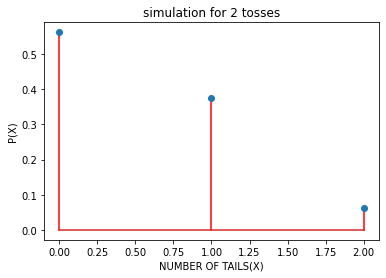
\includegraphics[width=0.4 \textwidth]{rvspt2.png}
 \end{figure} 
\begin{figure}[ht]
   % \centering
    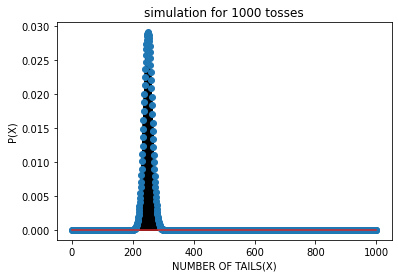
\includegraphics[width=0.4 \textwidth]{rvsptt.png}
    
\end{figure}




\end{document}
